\chapter{Process}
\label{chap:process}

\noindent\textit{Readers without an ML/AI background may find the brief explanation of concepts from this chapter in Appendix~\ref{appendix:concepts}.}

\section{Dataset Exploration}

First, the Spr\r{a}kbanken S\'{a}mi OCR corpus~\cite{sprakbanken_dataset,enstad2025} from Hugging Face was analysed. It consists of train/validation/test splits (307k/40.8k/84.5k rows), ment for fitting OCR models for North S\'{a}mi, Lule and Inari S\'{a}mi. Each sample is a single synthetically rendered text line paired with its ground truth transcription, e.g.\ those shown in Figure~\ref{fig:report-samples}. The line by line format meant that line detection and layout analysis were outside the scope of the model. The OCR goal was to transcribe the line of text into a string.
Extracted vocabulary yielded a \charsetSize{} symbol charset (\numCharsVocab{} characters plus one CTC blank token) later used by the CTC head. The computed word and letter frequencies are rendered as the clouds in Figure~\ref{fig:report-corpus}. 
Two observations from this step shaped later decisions. The conjunction \textit{ja} (``and'') dominates the word distribution, foreshadowing the conjunction splitting preprocessing. The seven special characters appear at non-negligible frequencies.

\begin{figure}[h]
\centering
\begin{tabular}{c}
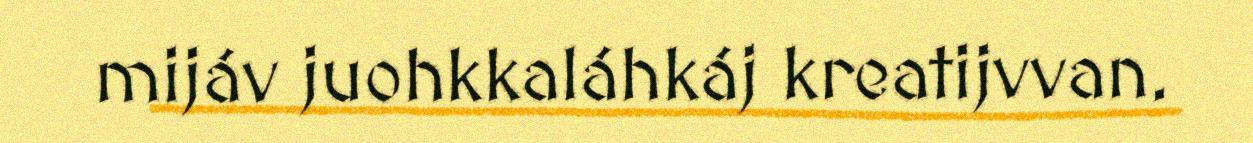
\includegraphics[width=0.92\linewidth]{figures/correct2.jpg} \\[2pt]
\footnotesize \textit{mij\'{a}v juohkkal\'{a}hk\'{a}j kreatijvvan.} \\[10pt]
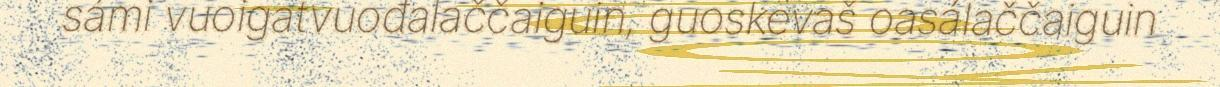
\includegraphics[width=0.92\linewidth]{figures/example1.jpg} \\[2pt]
\footnotesize \textit{sámi vuoigatvuođalaččaiguin, guoskevaš oasálaččaiguin} \\
\end{tabular}
\caption{Two Spr\r{a}kbanken synthetic samples shown as the model sees them.The rendering varies font, spacing, slight noise and background to simulate scanned text appearance.}
\label{fig:report-samples}
\end{figure}

\begin{figure}[h]
\centering
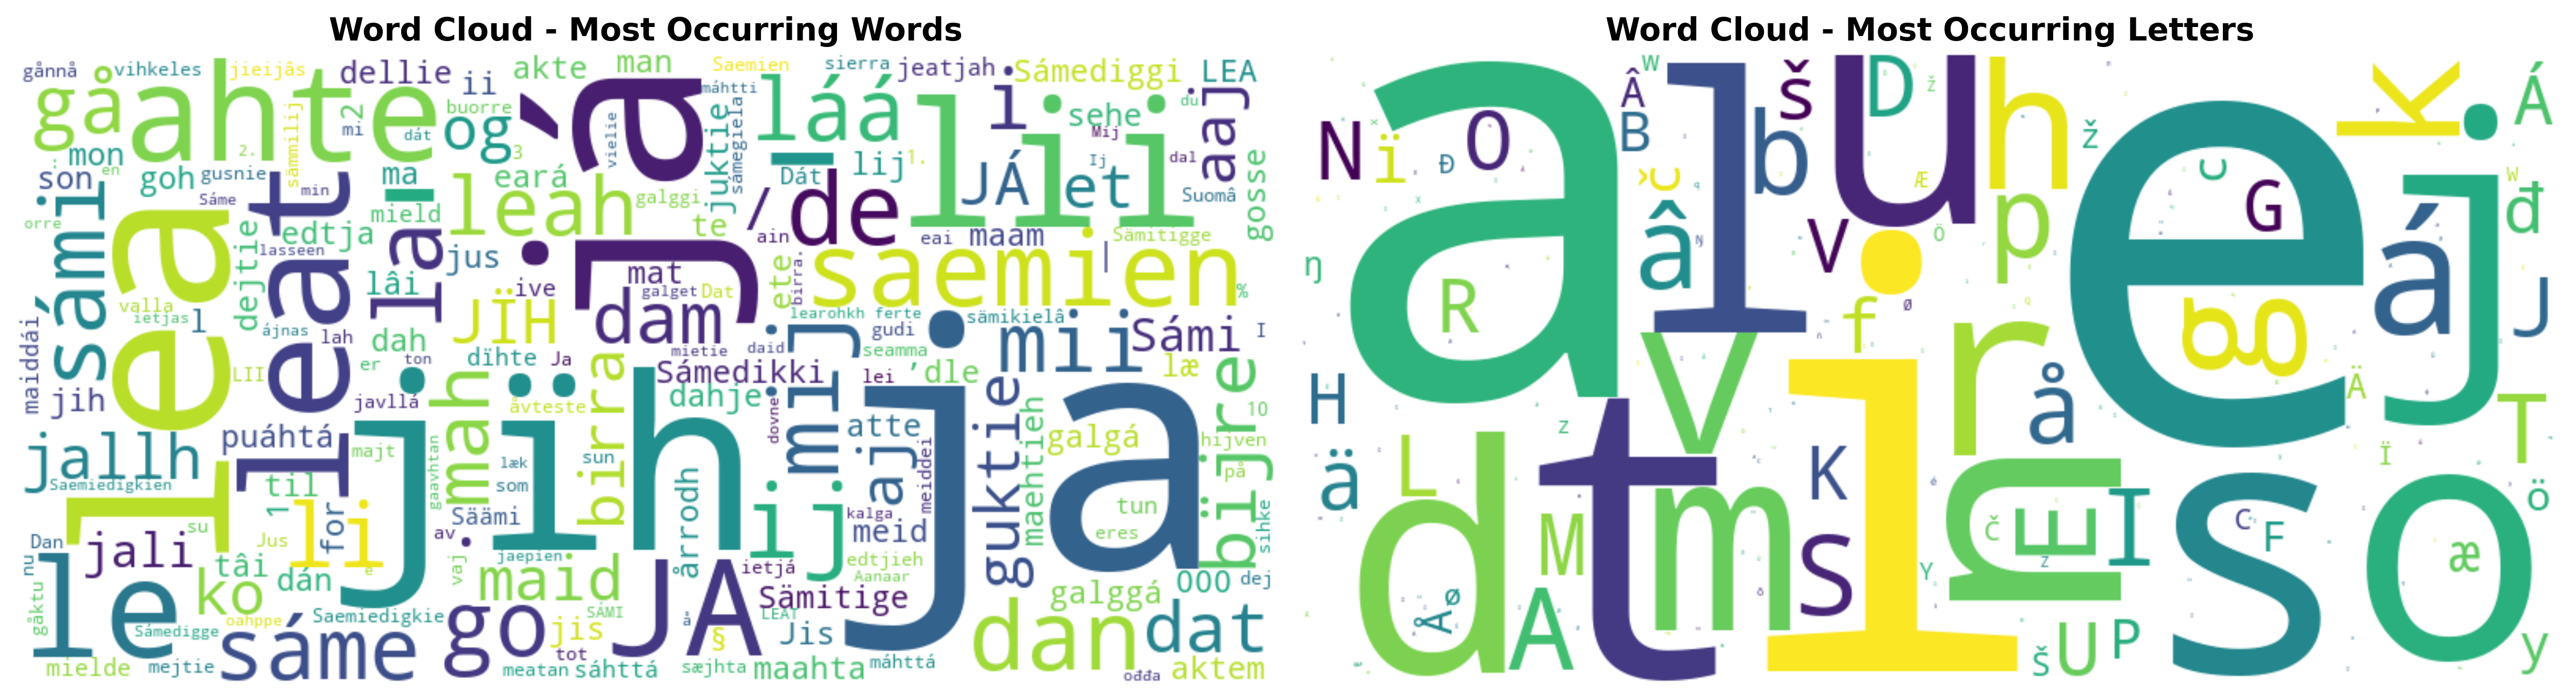
\includegraphics[width=\linewidth]{figures/word_letter_clouds.png}
\caption{Word and letter clouds of the Spr\r{a}kbanken North S\'{a}mi training corpus.}
\label{fig:report-corpus}
\end{figure}

\section{Corpus Building Detour}
\label{sec:corpus-detour}

A small detour was taken during the early stages of the project to assess whether a parallel English S\'{a}mi corpus could be built from Turi's \textit{Muitalus s\'{a}miid birra} (1910). The idea was to explore a possibility of training a MT solution using the yielded corpora (e.g. Gated Recurrent Unit (GRU) Network) Both versions of the book were obtained as PDFs, one in North S\'{a}mi (Friis' orthography), the other in English (translated and edited by Thomas A. DuBois), alongside an already parsed, sentence split S\'{a}mi version from the Giellatekno website.

The PDFs are parsed with \texttt{pdfminer}, split into sentences with NLTK, and aligned with a custom TUI tool that supports manual approval (See Figure~\ref{fig:alignment-tool}), deletion, and merging of sentence pairs. Due to time constraints, the tool was ultimately not used to generate a full bilingual corpus, instead, it produced a small evaluation set of \bookTestSamples{} synthetic renderings of the S\'{a}mi sentences, which became the out of domain test set in the IISA paper.

\begin{figure}[h]
\centering
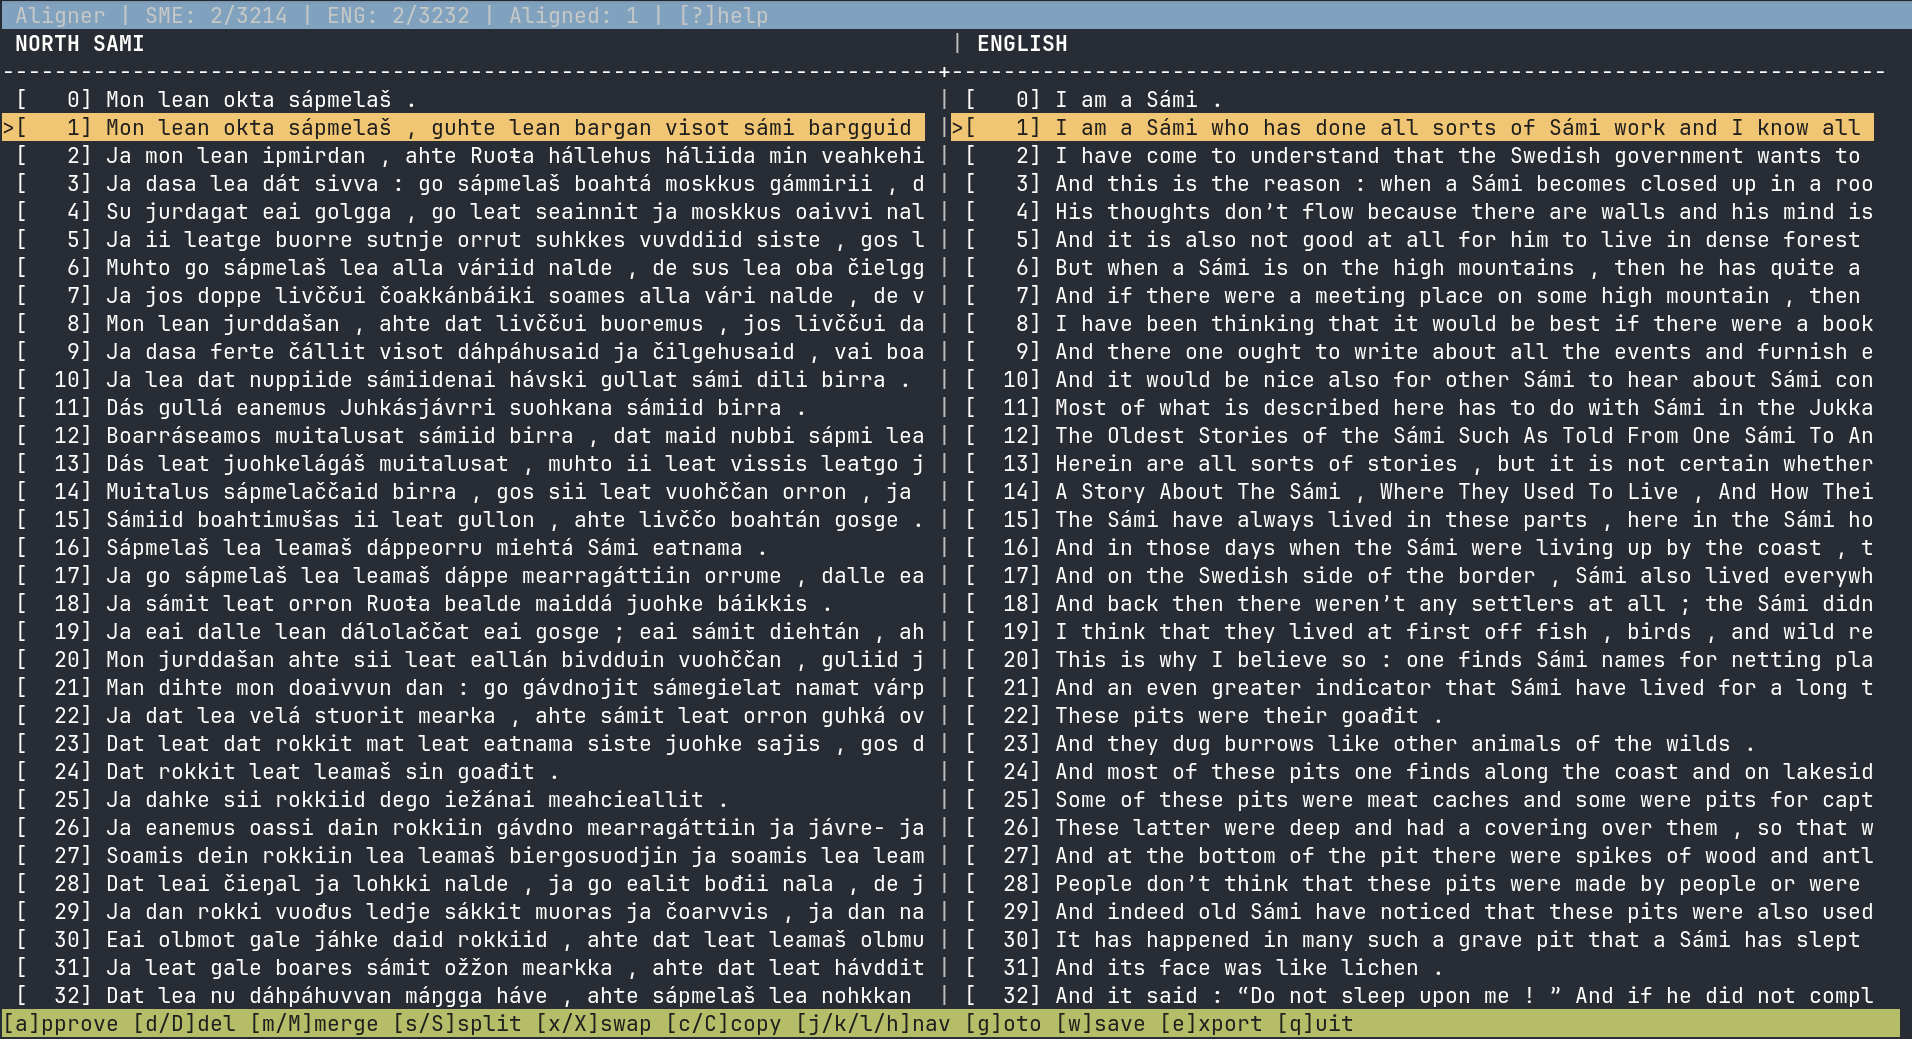
\includegraphics[width=\linewidth]{figures/alignment-tool.png}
\caption{Alignment CLI tool for parallel corpora generation from two sources.}
\label{fig:alignment-tool}
\end{figure}

\section{Training Pipeline Overview}
\label{sec:pipeline-overview}

The modular OCR pipeline consists of three slots: a \emph{backbone}, an \emph{encoder} and a \emph{decoder}. Each slot is easily swappable, yielding 15 distinct configurations in total: 5 backbones (SimpleCNN, VGG16, VGG19, ResNet50, ResNet101) $\times$ 3 encoders (none, BiLSTM, Transformer), with a fixed CTC decoder across all variants. A training queue runs configurations consecutively without manual intervention, logging each step and storing checkpoints and outputs in a structured way for monitoring and debugging. The modular design also leaves room for future extensions, such as a post correction module or a scan quality classifier.

This layout is inspired by Shi et al.'s CRNN~\cite{shi2017crnn}: a CNN backbone extracts spatial features, a sequence encoder adds temporal context, and a CTC head maps the encoded sequence to characters. Each component is explained in more detail below.

\subsection{Backbone}
\label{subsec:backbone}

The backbone slot contains the CNN feature extractor, which processes the input image into a sequence of column features. The proposed lightweight variant is a 7 layer SimpleCNN trained from scratch, while the comparison variants use ImageNet pretrained VGG16, VGG19, ResNet50 and ResNet101 backbones with differential learning rates to preserve pretrained features.

\subsection{Encoder}
\label{subsec:encoder}

The encoder slot contains the sequence modelling component, which captures contextual dependencies between characters. The options are a 2 layer BiLSTM, a Transformer encoder block, or no encoder (direct CNN to CTC). This allowed to isolate the contribution of explicit sequence modelling on top of the per column CNN features.

\subsection{Decoder}
\label{subsec:decoder}

The decoder slot contains the transcription head, which maps the encoded features to character probabilities. A CTC decoder \cite{graves2006ctc} is used across all configurations, which allows for training without explicit character level alignment and handles variable length outputs. This fixed decoder setup ensures that differences in performance can be attributed to the backbone and encoder choices.

\section{Comparison}
\label{sec:comparison}

The modular pipeline allowed for a systematic comparison of the CNN based variants against the transformer based models. The comparison benchmark was run on CPU to reflect realistic deployment conditions, and evaluated on the same test set using consistent metrics (CER, WER, exact match accuracy).

Due to limited accessibility to uCloud resources only the following variants were trained: \texttt{ctc\_simple} (the lightweight 7 layer SimpleCNN trained from scratch), \texttt{ctc\_vgg16} and \texttt{ctc\_vgg19} (ImageNet pretrained VGG backbones with differential learning rates), and \texttt{ctc\_resnet50} (ImageNet pretrained ResNet50). The \texttt{ctc\_resnet101} variant was gated on the ResNet50 results. Per epoch time on the V100 was $\sim$19~minutes for the VGG pair and $\sim$76~minutes for ResNet50, so a full 100 epoch run would have occupied the GPU for $\sim$32~hours (VGG) or $\sim$5~days (ResNet50). 
In practice all three pretrained variants triggered early stopping well before that: \texttt{ctc\_vgg16} at 52~epochs, \texttt{ctc\_vgg19} at 63~epochs, and \texttt{ctc\_resnet50} at 37~epochs ($\sim$48~hours), with validation CER stuck around 0.69 to 0.73 at early stopping (ResNet50's final test CER of 0.753 reflects continued degradation past that point, see Section~\ref{sec:main-result}). The compute budget made it impossible to commit further.

\section{The lightweight CNN-CTC variant}
\label{sec:lightweight-backbone}

The headline lightweight variant, \texttt{ctc\_simple}, uses a 7 layer SimpleCNN backbone trained from scratch, no encoder and a CTC head over the \charsetSize{} symbol vocabulary. The architecture is shown in Figure~\ref{fig:report-architecture}.

\begin{figure}[h]
\centering

\includegraphics[width=\linewidth, height=0.8\textheight, keepaspectratio]{figures/architecture_tikz.pdf}
\caption{Modular OCR pipeline used in the IISA paper. The lightweight \texttt{ctc\_simple} variant uses a 7 layer SimpleCNN backbone trained from scratch and a CTC head over the \charsetSize{} symbol vocabulary, the encoder slot is left empty.}
\label{fig:report-architecture}
\end{figure}

The SimpleCNN has 7 convolutional layers with following channel widths $64, 128, 256, 256, 512, 512, 512$, each followed by batch normalisation and a ReLU activation function.
Pooling is asymmetric: $2\times 2$ max pooling in the early layers progressively collapses both axes, while the later layers switch to $2\times 1$ pooling that keeps horizontal resolution intact, preserving the character ordering that the CTC head relies on. A final adaptive pool reduces feature map height to 1, yielding a sequence of column vectors. These are projected to \hiddenDim{} dimensions and passed directly to a linear head that maps to \charsetSize{} classes (\numCharsVocab{} characters plus the CTC blank) followed by LogSoftmax.
The full model has $\sim$\numParams{}M parameters.
It is trained with a CTC loss that marginalises over all valid character alignments and decoded greedily at inference time.
In practice it ran the full 100 epoch schedule at $\sim$8 minutes per epoch ($\sim$13 hours).


\section{Training Setup}
\label{sec:training-setup}

All CTC variants share the same training recipe with backbone specific overrides. The optimiser is AdamW with a base learning rate of $10^{-4}$ and weight decay $10^{-4}$ for \texttt{ctc\_simple}, reduced to $3\times 10^{-5}$ with a 0.1$\times$ differential multiplier on pretrained VGG and ResNet50 layers. The batch size is 32 for SimpleCNN and VGG, reduced to 16 for ResNet50 due to GPU memory. Training runs for up to 100 epochs with early stopping (patience 15 to 35 epochs, scaling with model size), \texttt{ReduceLROnPlateau} halves the learning rate when validation CER plateaus, and gradients are clipped to a max norm of 5.0 to stabilise the CTC loss.

The training data is the Spr\r{a}kbanken synthetic North S\'{a}mi OCR corpus~\cite{sprakbanken_dataset,enstad2025}, with \trainSamples{} samples in the training subset (90\% of the 307{,}387-sample training split) and roughly \hfValidationSamples{} held out for development. 


\section{Evaluation and End to End Pipeline}
\label{sec:evaluation-pipeline}

Evaluation is conducted on a \testSamples{} sample combined test set: \hfTestSamples{} held out samples from the Spr\r{a}kbanken validation split (in domain) and \bookTestSamples{} synthetic renderings of Turi's \turiYear{} \textit{Muitalus s\'{a}miid birra} (out of domain lexical content). Models are scored with character error rate (CER), word error rate (WER), exact match accuracy, and a normalised accuracy variant that removes punctuation and extra whitespaces, all computed as Levenshtein distance on raw UTF-8 strings. Per image inference time is measured on CPU to reflect realistic deployment conditions. The TrOCR variants are used as released by the National Library of Norway without additional fine tuning, while \texttt{ctc\_simple} is trained from scratch on the Spr\r{a}kbanken corpus. The benchmark compares a ready pretrained baseline against a purpose trained lightweight model.

The full end to end pipeline passes the OCR predictions into the TartuNLP North S\'{a}mi English machine translation API~\cite{tartunlp}, with the translated output scored against the English reference using BLEU, chrF~\cite{popovic2015chrf}, and TER (See Figure~\ref{fig:ocr-mt-pipeline}).

\section{Conjunction Splitting Experiment}
\label{sec:conjunction-split-process}

The experiment surfaced from the benchmark results. Per sentence error analysis on both \texttt{ctc\_simple} and the strongest TrOCR variants showed a steep accuracy drop beyond roughly \sentenceLengthThreshold{} characters, caused by the fixed \preprocessingImgWidth{} px input width cutoff. Referencing the most frequently used words in the dataset (Figure~\ref{fig:report-topwords})  where the conjunction \textit{ja} dominated the distribution suggested that splitting long inputs at North S\'{a}mi conjunction boundaries (\textit{ja} ``and'', \textit{muhto} ``but'', \textit{dahje} ``or'', \textit{go} ``when/because'', \textit{ahte} ``that'', \textit{jos} ``if'') before OCR and rejoin the predictions afterwards, might mitigate that issue.

\begin{figure}[h]
\centering
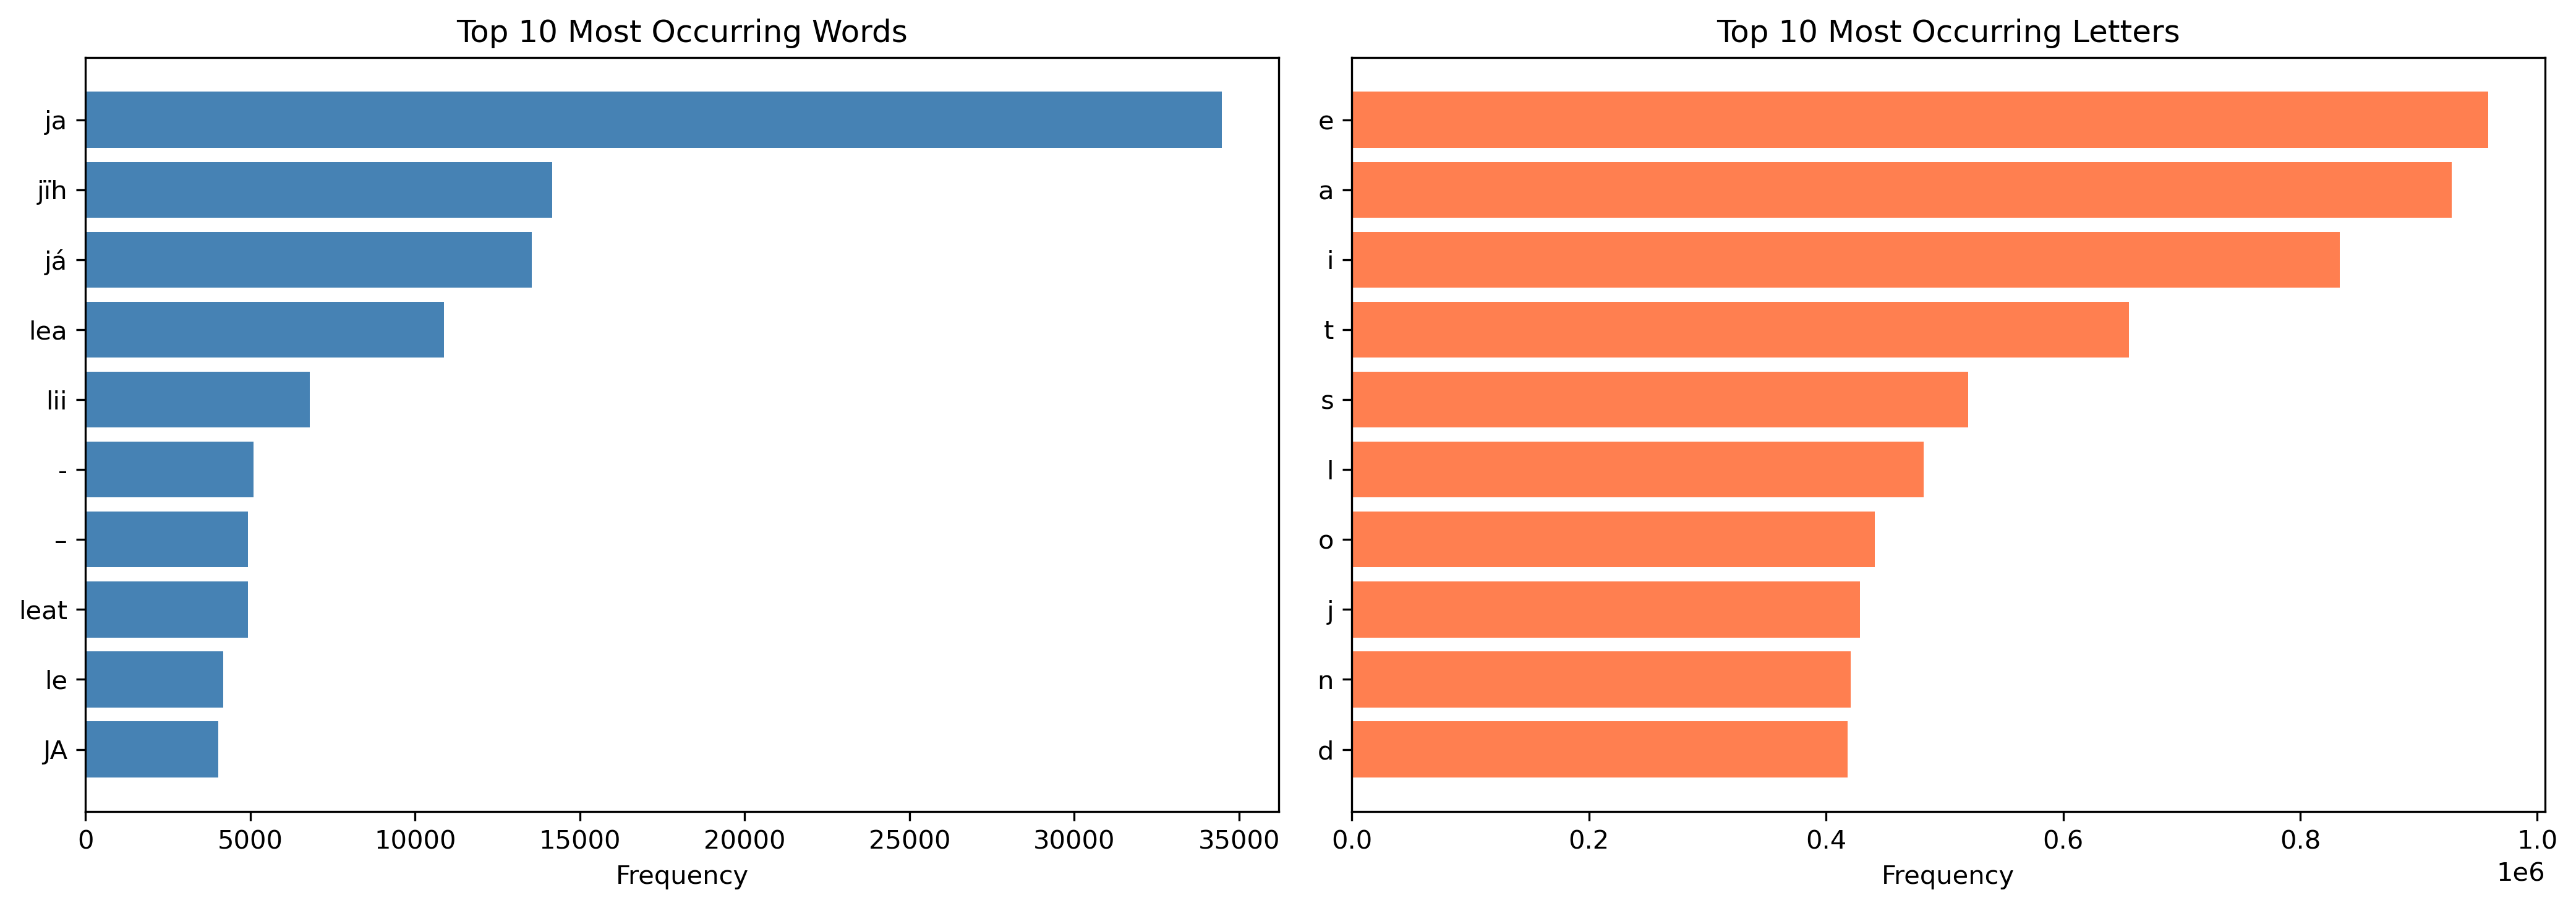
\includegraphics[width=\linewidth]{figures/top_words_letters_bars.png}
\caption{Top 10 most frequent words (left) and characters (right) in the Spr\r{a}kbanken North S\'{a}mi training corpus. The conjunction \textit{ja} (``and'') is by far the most frequent token, motivating conjunction based segmentation.}
\label{fig:report-topwords}
\end{figure}

More specifically, every input sentence longer than \sentenceLengthThreshold{} characters is scanned for these conjunction tokens by a case insensitive word boundary regex matching (the implementation also extends to multi-word and subordinate variants such as \textit{ovdal go} ``before'' and \textit{dasgo} ``because''), with the multi-word forms being matched greedily before their single-word counterparts to avoid double counting. The text is split immediately \textit{before} each matched conjunction so the connective stays attached to its following clause, and a minimum segment length of 20 characters guards against over splitting when there are many conjunctions close to eachother. Each resulting text segment is then re-rendered as a fresh synthetic line image through the same generator used for the evaluation out-of-domain data, passed independently through \texttt{ctc\_simple}, and the per segment predictions are joined with single space to form the final transcription. The benchmark compares per sample CER on the long sentence subset of the test set before and after splitting, with statistical significance estimated via a paired test and effect size reported as Cohen's $d$.

\begin{figure}[h]
\centering
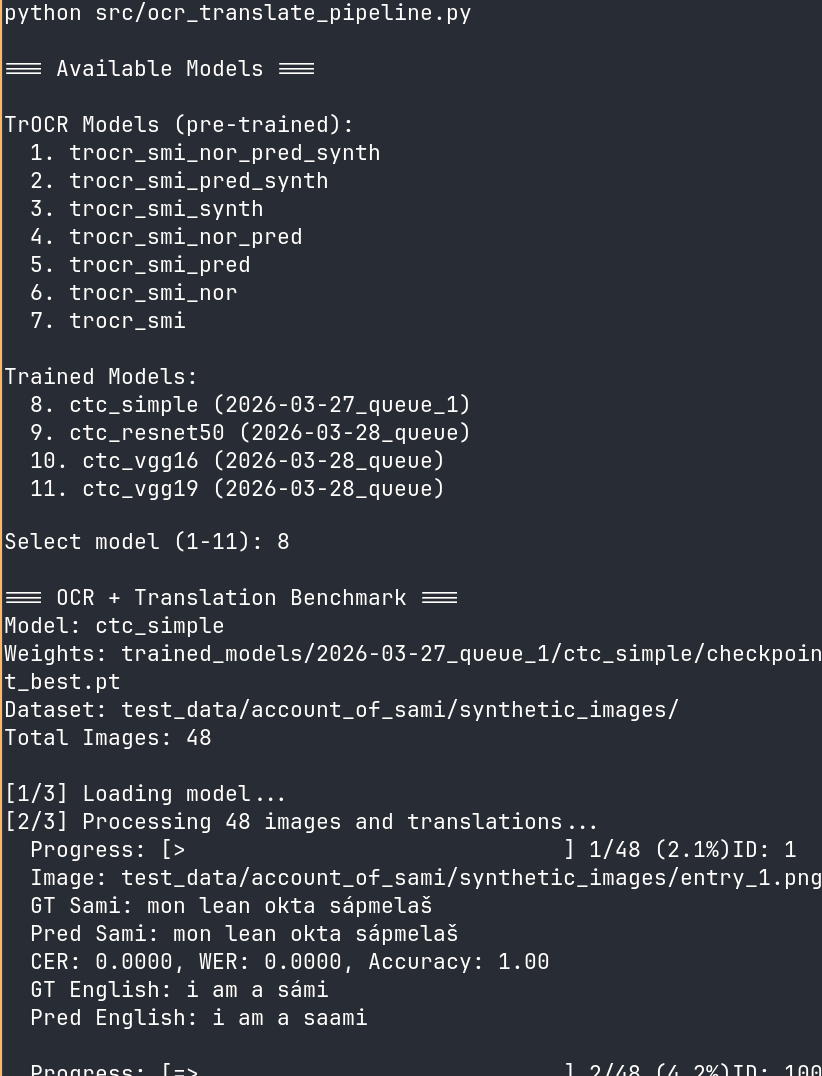
\includegraphics[width=\linewidth]{figures/ocr-mt-pipeline.png}
\caption{CLI tool for running the end to end OCR$\rightarrow$translation pipeline. The user selects the OCR model and dataset, and the tool reports both OCR accuracy metrics (CER, WER) and translation quality metrics (BLEU, chrF, TER) on the translated output.}
\label{fig:ocr-mt-pipeline}
\end{figure}